
\plain{Answers: Organic Best Of vs Bandit Best Of}




\begin{frame}[fragile]
  \frametitle{Answer Q1 Histogram of product popularity}
\begin{small}
\begin{verbatim}
  clicks = np.zeros(NumberOfProducts)
  bandits = data[data['z'] == 'bandit']
  for product_id in range(NumberOfProducts):
      actions = bandits[bandits['a'] == product_id]
      clicks[product_id] = np.sum(actions[actions['c'] == 1]['c'])
      
  print("Clicks: ", clicks)
  
  _, ax = plt.subplots()
  ax.set_title('Histogram of Clicks per Product')
  
  ax.bar(range(NumberOfProducts), clicks)
  plt.show()
\end{verbatim}
\end{small}
\end{frame}


\begin{frame}[fragile]
  \frametitle{Answer Q2 Non-personalized CTR}
\begin{tiny}
\begin{verbatim}
  from scipy.stats.distributions import beta

  clicks = np.zeros(NumberOfProducts)
  impressions = np.zeros(NumberOfProducts)
  lower_errors = np.zeros(NumberOfProducts)
  upper_errors = np.zeros(NumberOfProducts)
  bandits = data[data['z'] == 'bandit']
  for product_id in range(NumberOfProducts):
      actions = bandits[bandits['a'] == product_id]
      clicks[product_id] = np.sum(actions[actions['c'] == 1]['c'])
      impressions[product_id] = sum(actions['a']==product_id)
\end{verbatim}
\end{tiny}
\end{frame}

\begin{frame}[fragile]
  \frametitle{Answer Q3 Best of CTR}
\begin{verbatim}
  top_ctr_item = np.argmax(clicks/impressions)
\end{verbatim}
\end{frame}


\begin{frame}[fragile]
  \frametitle{Answer Q4 most views}
\begin{verbatim}
  top_viewed_item = np.argmax(views)
\end{verbatim}
\end{frame}




\begin{frame}[fragile]
  \frametitle{}
  \begin{small}
\begin{verbatim}
data = deepcopy(env).generate_logs
        (ABTestNumberOfUsers, agent=organic_counter_agent)
\end{verbatim}
\end{small}
\end{frame}




\begin{frame}
\frametitle{Organic Best-Of vs Bandit Best-Of}

As the logging policy chose its actions uniformly at random, we can see that all items were recommended roughly the same number of times.

\begin{figure}[h!]
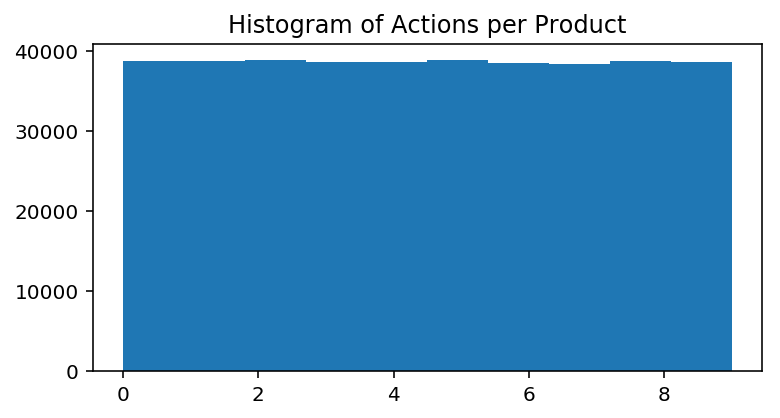
\includegraphics[scale=0.4]{images/organic_bestof0.png}
\centering
\label{motex1}
\end{figure}
\end{frame}

\begin{frame}
\frametitle{Organic Best-Of vs Bandit Best-Of}

We can examine the click through rate of each action under this policy, we see that action 5, 2 and 9 have high click through rates.

\begin{figure}[h!]
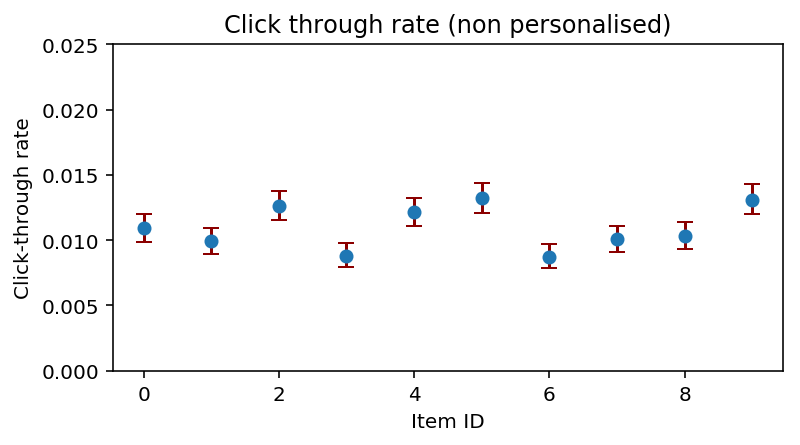
\includegraphics[scale=0.4]{images/organic_bestof1.png}
\centering
\label{motex1}
\end{figure}
\end{frame}

\begin{frame}
\frametitle{Organic Best-Of vs Bandit Best-Of}


\begin{figure}[h!]

  We can also examine which items are organically the most popular, this time we see that item 4 and item 9 are the most popular.

  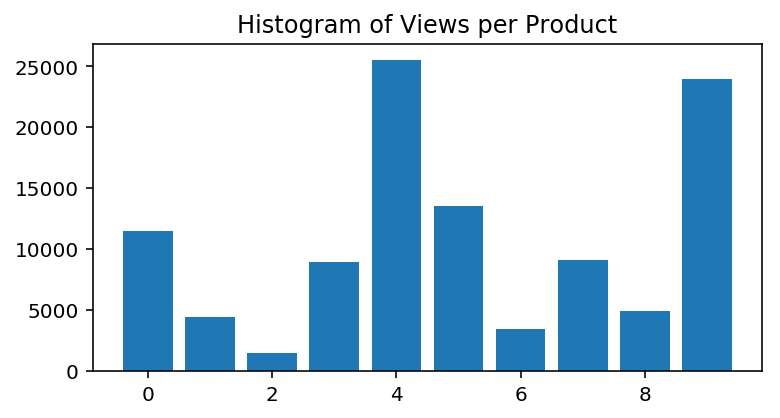
\includegraphics[scale=0.4]{images/organic_bestof2.png}
\centering
\label{motex1}
\end{figure}
\end{frame}

\begin{frame}
\frametitle{Organic Best-Of vs Bandit Best-Of}

If we plot popularity vs non-personalized click through rate we see some kind of relationship, but the correlation is noisy.


\begin{figure}[h!]
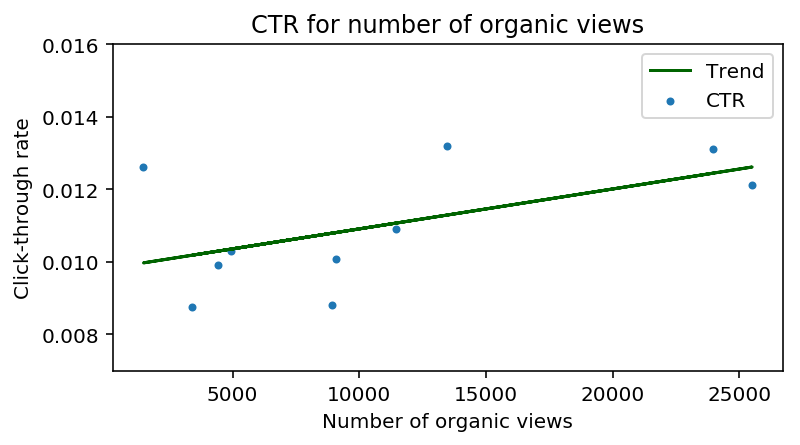
\includegraphics[scale=0.4]{images/organic_bestof3.png}
\centering
\label{motex1}
\end{figure}
\end{frame}

\begin{frame}
\frametitle{Organic Best-Of vs Bandit Best-Of}

A bandit best-of agent always recommends the highest ctr product (product 5).  An organic best-of always recommends the most frequently viewed product (product 4).  A simulated AB test shows using the bandit best-of yields a better result.

\end{frame}

\begin{frame}
\frametitle{Organic Best-Of vs Bandit Best-Of}
  
\begin{figure}[h!]
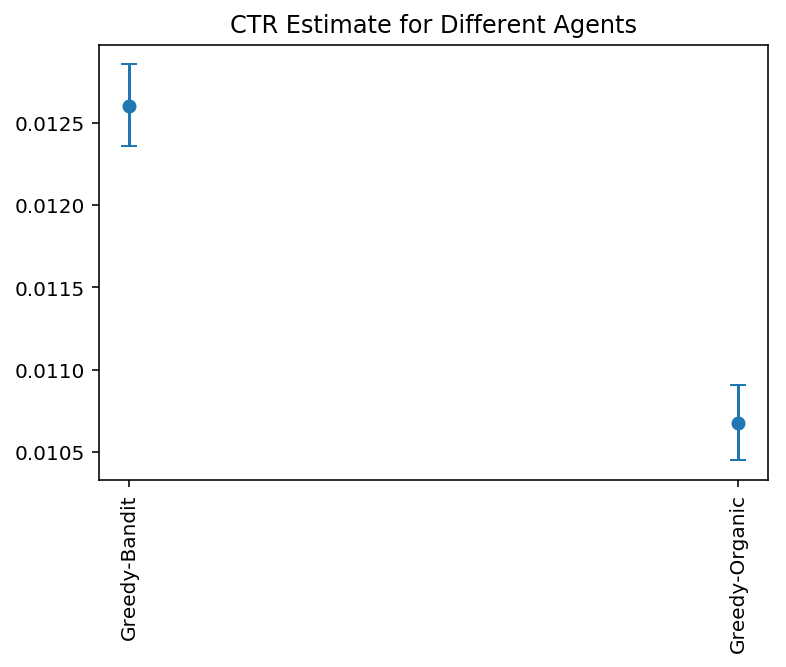
\includegraphics[scale=0.4]{images/bestof.png}
\centering
\label{motex1}
\end{figure}

\pause
Personalization of course will result in a better result still.
\end{frame}


\plain{Answers: Evaluate an organic agent using the Bandit Signal}



\begin{frame}[fragile]
  \frametitle{Answer}
\begin{tiny}  
\begin{verbatim}
def observe(self, observation):
  for session in observation.sessions():
      self.user_embedding += self.embeddings[session['v'],:]
      self.history_length += 1

def act(self, observation, reward, done):
  """Act method returns an Action based on current observation and past history"""
  self.observe(observation)
  next_item_score = np.matmul(self.embeddings,self.user_embedding/self.history_length)

  action = np.argmax(next_item_score)        
  prob = np.zeros_like(next_item_score)
  prob[action]=1.0
  return {
      **super().act(observation, reward, done),
      **{
          'a': action,
          'ps': 1.0,
          'ps-a': prob,
      },
  }
\end{verbatim}
\end{tiny}
\end{frame}

